\chapter{Topology}
\section{Topological spaces}
\begin{propositionenv}
    Let $X$ be a set and for any $x\in X$, let $\mathcal{G}_x$ be a filter contained in the principal filter of $\{x\}$ ($\forall U\in \mathcal{G}_x,\ x\in U$). Denote by $\mathscr{T}$ the set 
    $$\{U\in \wp(X) \mid \forall x\in U, U\in\mathcal{G}_x\}.$$
    Then the following conditions are satisfied.
    \newline
    (1) $\{\varnothing, X\} \subseteq \mathscr{T}$.
    \newline
    (2) If $(U_1,U_2)\in \mathscr{T}^2$, then $U_1\cap U_2\in \mathscr{T}$.
    \newline
    (3) If $I$ is a set and $\left(U_i\right)_{i\in I}\in \mathscr{T}^I$, then $\dis \bigcup_{i\in I}U_i\in \mathscr{T}$.
    \newline
    Moreover, $\forall x\in X,\ \mathcal{B}_x=\{U\in \mathscr{T}\mid x\in U\}$ is a filter basis contained in $\mathcal{G}_x$. It generates $\mathcal{G}_x$ if the following condition is satisfied:
    $$\forall U\in \mathcal{G}_x,\ \exists V\in \mathcal{G}_x,\ V\subseteq U \text{ and } \forall y\in V,\ V\in \mathcal{G}_y.$$
\end{propositionenv}
\begin{proofenv}
    \ \newline
    (1) $\dis \varnothing \in \mathscr{T}, X\in \bigcap_{x\in X}\mathcal{G}_x$.
    \newline
    (2) $\forall x\in U_1\cap U_2,\ U_1\in \mathcal{G}_x,\ U_2\in \mathcal{G}_x$, so $U_1\cap U_2\in \mathcal{G}_x$.
    \newline
    (3) Let $\dis U=\bigcup_{i\in I}U_i$. $\forall x\in U,\ \exists i\in I,\ x\in U_i$, so $U_i\in \mathcal{G}_x$. Since $U\supseteq U_i$, so $U\in\mathcal{G}_x$.
    $$\mathcal{B}_x:=\{U\in \mathscr{T}\mid x\in U\}.$$
    If $U\in \mathcal{B}_x$, then $x\in U$, so $U\in \mathcal{G}_x$. Hence $\mathcal{B}_x\subseteq\mathcal{G}_x$. If $(U,V)\in \mathcal{B}_x^2$, then $U\cap V\in \mathscr{T}$, and $x\in U\cap V$. So $U\cap V\in \mathcal{B}_x$. So $\mathcal{B}_x$ is a filter basis. Suppose the condition is satisfied. For any $U\in \mathcal{G}_x,\ \exists V\in \mathcal{G}_x\cap\mathscr{T}$, such that $V\subseteq U$. Note that $V\in \mathcal{B}_x$, so $\mathcal{G}_x$ is generated by $\mathcal{B}_x$.
\end{proofenv}
\begin{definitionenv}
    Let $X$ be a set. We call \textbf{topology} on $X$ any subset $\mathscr{T}$ of $\wp(X)$ that satisfies the following conditions:
     \newline
    (1) $\{\varnothing, X\} \subseteq \mathscr{T}$.
    \newline
    (2) If $(U_1,U_2)\in \mathscr{T}^2$, then $U_1\cap U_2\in \mathscr{T}$.
    \newline
    (3) For any set $I$,  $ \forall \left(U_i\right)_{i\in I}\in \mathscr{T}^I$, then $\dis \bigcup_{i\in I}U_i\in \mathscr{T}$.
    \newline
    $(X,\mathscr{T})$ is called a \textbf{topological space}.
    \newline
    If $\forall x\in X,\ \mathcal{B}_x$ is a filter basis of $X$ contained in the principal filter of $\{x\}$, then 
    $$\mathscr{T}=\{U\in \wp(X)\mid \forall x\in U,\ \exists V_x\in \mathcal{B}_x,\ V_x\subseteq U\}$$
    is a topology on $X$, called the \textbf{topology generated by} $(\mathcal{B}_x)_{x\in X}$. More generally, if $\forall x\in X,\ S_x $ is a subset of the principal filter of $\{x\}$ and $\mathcal{G}_x$ is the filter generated by $S_x$, then we say that 
    $$\mathscr{T}=\{U\in\wp(X)\mid \forall x\in U,\ U\in \mathcal{G}_x\}$$
    is the topology generated by $(S_x)_{x\in X}$.

\end{definitionenv}
\begin{exampleenv}
    \ \newline
    (1) Let $\mathcal{G}_x=\{X\}$. The topology by $\left(\mathcal{G}_x\right)_{x\in X}$ is $\{\varnothing,X\}$, called the \textbf{trivial topology} on $X$.  
    \newline
    (2) Let $\mathcal{G}_x=\mathcal{F}_{\{x\}}$ be the principal filter. The topology generated by $\left(\mathcal{G}_x\right)_{x\in X}$ is $\wp(X)$. This topology is called the \textbf{discrete topology} on $X$.
    \newline
    (3) Let $(X,\mathrm{d})$ be a semimetric space. 
    $$\mathrm{d}:X\times X\longrightarrow \mathbb{R}_{\ge 0},\  \mathrm{d}(x,y)=\mathrm{d}(y,x),\ \mathrm{d}(x,z)\le \mathrm{d}(x,y)+\mathrm{d}(y,z),\ \mathrm{d}(x,x)=0.$$
    $\forall \varepsilon>0,\ \forall x\in X$, let $B(x,\varepsilon)=\{y\in X\mid \mathrm{d}(x,y)<\varepsilon\}$, $\{B(x,\varepsilon)\mid \varepsilon\in \RR_{>0}\}=: \mathcal{B}_x$ is a filter basis on $X$, $\mathcal{B}_x$ is contained in the principal filter of $\{x\}$. The topology 
    $$\mathscr{T}=\{U\in \wp(X)\mid \forall x\in U,\ \exists \varepsilon\in \RR_{>0},\ B(x,\varepsilon)\subseteq U\}$$
    is called the \textbf{topology induced by the semimetric $\mathrm{d}$}.
    \newline
    (4) Let $(G,\le )$ be a totally ordered set $\forall x\in G$, let $S_x=\{G_{>a}\mid a<x\}\cup \{G_{<b}\mid x<b\}$
\end{exampleenv}
\begin{propositionenv}
    $\forall x\in X,\ \forall \varepsilon\in \RR_{>0}, B(x,\varepsilon)\in \mathscr{T}$.
\end{propositionenv}
\begin{proofenv}
    $\forall y\in B(x,\varepsilon),\ \mathrm{d}(x,y)<\varepsilon$. Let $r=\varepsilon-\mathrm{d}(x,y)>0$, we claim that $B(y,r)\subseteq B(x,\varepsilon)$. Let $z\in B(y,r), \ \mathrm{d}(y,z)<r$. Hence,
    $$\mathrm{d}(x,z)\le \mathrm{d}(x,y)+\mathrm{d}(y,z)<\mathrm{d}(x,y)+r=\mathrm{d}(x,y)+\varepsilon -\mathrm{d}(x,y)=\varepsilon.$$
\end{proofenv}
\begin{remark}
    On $\RR$, one has a metric 
    $$\mathrm{d}: \RR\times \RR\longrightarrow \RR_{\ge 0},$$
    $$\left(a,b\right)\longmapsto |a-b|.$$
    $$B(x,\varepsilon)=\interval[open]{x-\varepsilon}{x+\varepsilon}.$$
    $$\mathcal{B}_x=\{\interval[open]{x-\varepsilon}{x+\varepsilon}\mid \varepsilon\in \RR_{>0}\}.$$
    Let $\mathscr{T}_\mathrm{d}$ be the topology generated by $(\mathcal{B}_x)_{x\in \RR}$. Let $\mathscr{T}$ be the order topology generated by $\left(S_x\right)_{x\in \RR}$, where 
    $$S_x:=\{\RR_{>a}\mid a<x\}\cup \{\RR_{<b}\mid x<b\}.$$
\end{remark}
\begin{propositionenv}
    For any $x\in \RR$, $\mathcal{F}(\mathcal{B}_x)=\mathcal{F}(S_x)$.
\end{propositionenv}
\begin{proofenv}
    $\forall \varepsilon>0,\ \interval[open]{x-\varepsilon}{x+\varepsilon}=\RR_{<x+\varepsilon}\cap \RR_{>x-\varepsilon}\in \mathcal{F}(S_x)$. So $\mathcal{F}(\mathcal{B}_x)\subseteq \mathcal{F}(S_x)$.
    $$\forall a\in \RR,\ a<x,\ \RR_{>a}\supseteq \interval[open]{a}{2x-a}=\interval[open]{x-(x-a)}{x+(x-a)},\ \RR_{>a}\in \mathcal{F}(\mathcal{B}_x).$$
    $$\forall b\in \RR, b>x,\RR_{<b}\supseteq \interval[open]{2x-b}{b}=\interval[open]{x+(b-x)}{x+(b-x)},$$
    So, $\RR_{<b}\subseteq\mathcal{F}(\mathcal{B}_x)$. Hence $S_x\subseteq \mathcal{F}(\mathcal{B}_x)$, which leads to $\mathcal{F}(S_x)\subseteq\mathcal{F}(\mathcal{B}_x)$.
\end{proofenv}
\begin{definitionenv}
    Let $(X,\mathscr{T})$ be a topological space. For any $x\in X$ and any $V\in \wp(X)$, if there exists $U\in \mathscr{T}$ such that $x\in U\subseteq V$, then we say that $V$ is a \textbf{neighborhood of $x$}. We call \textbf{open subset} of $X$ any subset of $X$ that belongs to $\mathscr{T}$. If $U\in \mathscr{T}$, such that $x\in U$, we say that $U$ is an \textbf{open neighborhood of $x$}. We denote by $\mathcal{V}_x(\mathscr{T})$ the set of all neighborhoods of $x$.
\end{definitionenv}
\begin{propositionenv}
    $\mathcal{V}_x(\mathscr{T})$ is a filter on $X$ contained in the principal filter of $\{x\}$. Moreover, the topology generated by $\left(\mathcal{V}_x(\mathscr{T})\right)_{x\in X}$ identifies with $\mathscr{T}$.
\end{propositionenv}
\begin{proofenv}
    \ \newline
    (1) If $(V_1,V_2)\in \mathcal{V}_x(\mathscr{T})^2,\ \exists (U_1,U_2)\in \mathscr{T}^2$, such that $x\in U_1\subseteq V_1,\ x\in U_2\subseteq V_2$. Hence, $x\in U_1\cap U_2\subseteq V_1\cap V_2$, so $V_1\cap V_2\in \mathcal{V}_{x}(\mathscr{T})$.
    \newline
    (2) If $V\in \mathcal{V}_x(\mathscr{T})$, $W\in \wp(X),\ V\subseteq W$. $\exists U\in \mathscr{T}$, $x\in U\subseteq V\subseteq W$, so $W\in \mathcal{V}_x(\mathscr{T})$. Let $\mathscr{T}'$ be the topology generated by $\left(\mathcal{V}_x(\mathscr{T})\right)_{x\in X}$. By definition,
    $$\mathscr{T}'=\{U\subseteq X\mid \forall x\in U, U\in \mathcal{V}_x(\mathscr{T})\}.$$
    For any $U\in \mathscr{T},\ \forall x\in U  $, $U$ is a open neighborhood of $x$, so $U\in \mathscr{T}'$. Let $U\in \mathscr{T}', \ \forall x\in U,\ \exists V_2\in \mathscr{T},\ x\in V_x\subseteq U$.
    $$U=\bigcup_{x\in U}\{x\}\subseteq \bigcup_{x\in U}V_x\subseteq U.$$
    $$U=\bigcup_{x\in U}V_x\in \mathscr{T}.$$
\end{proofenv}
\begin{propositionenv}
    Let $X$ be a set, $\left(\mathscr{T}_i\right)_{i\in I}$ be a family of topologies on $X$. Then 
    $$\mathscr{T}=\bigcap_{i\in I}\mathscr{T}_i$$
    is a topology on $X$.
\end{propositionenv}
\begin{proofenv}
    \ \newline
    (1) $\forall i\in I,\ \{\varnothing,X\}\subseteq \mathscr{T}_i$, so $\{\varnothing,X\}\subseteq \mathscr{T}$.
    \newline
    (2) If $(U_1,U_2)\in \mathscr{T}^2$, then for any $i\in I$, $\ U_1\cap U_2\in \mathscr{T}_i$, so $\dis U_1\cap U_2\in \bigcap_{i\in I}\mathscr{T}_i$.
    \newline
    (3) For any set $J$ and any $\left(U_j\right)_{j\in J}\in \mathscr{T}^J$, one has $\forall i\in I,\ \forall j\in J,\ U_j\in \mathscr{T}_i$, so
    $$\bigcup_{j\in J}U_j\in \mathscr{T}_i.$$
    Therefore, $$\bigcup_{j\in J}U_j\in \bigcap_{i\in I}\mathscr{T}_i.$$ 
\end{proofenv}
\begin{definitionenv}
    Let $S$ be a subset of $\wp(X)$, we denote by $\mathscr{T}_S$ the intersection of all topologies containing $S$, we call it the topology generated by $S$. 
\end{definitionenv}
\begin{definitionenv}
    \ \newline
    Let $\mathcal{B}$ be a subset of $\wp(X)$, we say that $\mathcal{B}$ is a topological basis if:
    \newline
    (1) $\dis X=\bigcup_{V\in \mathcal{B}}V$.
    \newline
    (2) $\forall (U,V)\in \mathcal{B}\times\mathcal{B},\ \forall x\in U\cap V,\ \exists W_x\in \mathcal{B},\ x\in W_x\subseteq U\cap V$.
\end{definitionenv}
\begin{definitionenv}
    Let $X$ be a set and $\mathscr{T}_1$ and $\mathscr{T}_2$ be two topologies on $X$. If $\mathscr{T}_1\subseteq\mathscr{T}_2$, we say that $\mathscr{T}_1$ is coarser than $\mathscr{T}_2$ and $\mathscr{T}_2$ is finer than $\mathscr{T}_1$. 
    
    If $S\subseteq\wp(X)$, we denote by $\mathscr{T}_S$ the intersection of all topology containing $S$. It is the coarsest topology containing $S$. 
    
    Let  $\mathcal{B}\subseteq \wp(X)$. If $\dis X=\bigcup_{V\in \mathcal{B}}V$ and $\forall (U,V)\in \mathcal{B}\times\mathcal{B},\ \forall x\in U\cap V,\ \exists W_x\in \mathcal{B},$ such that $x\in W_x\subseteq U\cap V$, we say that $\mathcal{B}$ is a \textbf{topological basis} on $X$.
\end{definitionenv}
\begin{propositionenv}
    Let $S$ be s subset of $\wp(X)$. Let 
    $$\mathcal{B}_S:=\{X\}\cup\left\{\bigcap_{i=1}^{n}A_i\mid n\in \NN_{\ge 1},\ (A_1,\dots,A_n)\in S^n\right\},$$
    then, $\mathcal{B}_S$ is a topological basis on $X$. Moreover, $\mathscr{T}_S=\mathscr{T}_{\mathcal{B}_S}$.
\end{propositionenv}
\begin{proofenv}
    Since $X\in \mathcal{B}_S$, $\dis\bigcup_{V\in \mathcal{B}_S}V=X$. Let $(U,V)\in \mathcal{B}_S\times\mathcal{B}_S$. If $U=X$, then $U\cap V=V\in \mathcal{B}_S$. Similarly, if $V=X$, then $U\cap V=U\in \mathcal{B}_S$. 

    If $U=A_1\cap\dots\cap A_n,\ V=B_1\cap\dots\cap B_m$, then $\{A_1,\dots, A_n,B_1,\dots,B_m\}\subseteq \mathcal{B}_S$. 
    $$U\cap V=A_1\cap\dots\cap A_n\cap B_1\cap\dots\cap B_m\in \mathcal{B}_S.$$
    Since $S\subseteq\mathcal{B}_S\subseteq\mathscr{T}_{\mathcal{B}_S}$, so $\mathscr{T}_{S}\subseteq\mathscr{T}_{\mathcal{B}_S}, \ X\in \mathscr{T}_S$. If $(A_1,\dots,A_n)\in S^n$, then $(A_1,\dots,A_n)\in\mathscr{T}_{\mathcal{B}_S}$. So $A_1\cap\dots\cap A_n\in \mathscr{T}_S$. Hence $\mathcal{B}_S\subseteq\mathscr{T}_{S}$. Therefore, $\mathscr{T}_{\mathcal{B}_S}\subseteq\mathscr{T}_S$, so $\mathscr{T}_{\mathcal{B}_S}=\mathscr{T}_S$.
\end{proofenv}
\begin{propositionenv}
    Let $\mathcal{B}$ be a topological basis on a set $X$. Then
    $$\mathscr{T}_{\mathcal{B}}=\left\{U\in\wp(X)\mid \exists \text{ a set }I \text{ and }(V_i)_{i\in I}\in \mathcal{B}^I, U=\bigcup_{i\in I}V_i\right\}.$$
\end{propositionenv}
\begin{proofenv}
    We denote by $\mathscr{T}$ te set 
    $$\{U\in \wp(X)\mid U\text{ can be written as as the union of a family sets in }\mathcal{B}\}.$$
    By definition, $\mathcal{B}\subseteq\mathscr{T}\subseteq\mathscr{T}_{\mathcal{B}}$. It remains to check that $\mathscr{T}$ is a topology.

    By definition, $X\in \mathscr{T},\ \varnothing\in \mathscr{T}$. Moreover, the union of a family of elements of $\mathscr{T}$ remains in $\mathscr{T}$. Let $\dis U=\bigcup_{i\in I}U_i$ and $\dis V=\bigcup_{j\in J}V_j$ be elements of $\mathscr{T}$, where, $U_i\in\mathcal{B}, V_{j}\in \mathcal{B}$. Then 
    $$ U\cap V=\bigcup_{(i,j)\in I\times J}\left(U_i\cap V_{j}\right).$$
    For any $x\in U_i\cap V_j$, $\exists W_x^{(i,j)}\in \mathcal{B},\ x\in W_x^{(i,j)}\subseteq U_i\cap V_j$. $\dis U_i\cap V_j=\bigcup_{x\in U_i\cap V_j}W_x^{(i,j)}$, so 
    $$U\cap V=\bigcup_{(i,j)\in I\times J}\bigcup_{x\in U_i\cap V_j}W_x^{(i,j)}.$$
\end{proofenv}


\section{Convergence}
We fix a topology space $(E,\mathscr{T})$, $l\in E$ and $S\subseteq \wp(E)$ that generates the filter $\mathcal{V}_l(\mathscr{T})$ of all neighborhood  of $l$.
\begin{definitionenv}
    Let $f:X\longrightarrow Y$ be a mapping. If $\mathcal{F}$ is a filter on $X$, we denote by $f_*(\mathcal{F})$ the set $\{B\subseteq Y\mid f^{-1}(B)\in\mathcal{F}\}$. 
\end{definitionenv}
\begin{propositionenv}
    $f_*(\mathcal{F})$ is a filter on $Y$.
\end{propositionenv}
\begin{proofenv}
    Let $(B_1,B_2)\in f_*(\mathcal{F})$,
    $$f^{-1}(B_1\cap B_2)=f^{-1}(B_1)\cap f^{-1}(B_2)\in \mathcal{F}.$$
    Let $B\in f_*(\mathcal{F}),\ C\supseteq B$. $f^{-1}(C)\supseteq f^{-1}(B)\in\mathcal{F}$, so $f^{-1}(C)\in \mathcal{F}$.
\end{proofenv}
\begin{propositionenv}
    Let $f:X\longrightarrow Y, \ g:Y\longrightarrow Z$, be mappings. $\mathcal{F}$ be a filter on $X$. Then
    $$\left(g\circ f\right)_{*}(\mathcal{F})=g_*(f_*(\mathcal{F})).$$
\end{propositionenv}
\begin{proofenv}
    \begin{align*}
        \left(g\circ f\right)_*(\mathcal{F})=&\{C\subseteq Z\mid \left(g\circ f\right)^{-1}(C)\in\mathcal{F}\}\\
        =&\{C\subseteq Z\mid f^{-1}(g^{-1}(C))\in \mathcal{F}\}\\
        =&\{C\subseteq Z\mid g^{-1}(C)\in f_*(\mathcal{F})\}\\
        =&g_*(f_*(\mathcal{F})).
    \end{align*}
\end{proofenv}
\begin{propositionenv}
    Let $\mathcal{B}$ be a filter basis in $X$,  $f:X\longrightarrow Y$ be a mapping and $\mathcal{F}$ be the filter generated by $\mathcal{B}$. Then $f(\mathcal{B}):\{f(U)\mid U\in \mathcal{B}\}$  is a filter basis on $Y$ and $f_*(\mathcal{F})$ is the filter generated by $f(\mathcal{B})$.
\end{propositionenv}
\begin{proofenv}
    Let $U$ and $V$ be elements of $\mathcal{B}$. Then $\exists W\in \mathcal{B},\ W\subseteq U\cap V$. Hence $f(W)\subseteq f(U\cap V)\subseteq f(U)\cap f(V).$ Moreover, for any $U\in\mathcal{B}$, $U\subseteq f^{-1}(f(U))$. So $f^{-1}(f(U))\in \mathcal{F}$. Therefore, $f(\mathcal{B})\subseteq f_*(\mathcal{F}) $. Let $A\in f_*(\mathcal{F})$. Then, $f^{-1}(A)\in \mathcal{F}$. So $\exists V\in \mathcal{B},\ V\subseteq f^{-1}(A)$. Hence $f(V)\subseteq A$. Therefore, $f_*(\mathcal{F})$ is a filter basis generated by $f_*(\mathcal{B})$
\end{proofenv}
\begin{definitionenv}
    Let $f:X\longrightarrow E$ be a mapping, $\mathcal{F}$ be a non-degenerate filter on $X$. If $f_*(\mathcal{F})\supseteq \mathcal{V}_l(\mathscr{T})$, we say that $f$ \textbf{converges} to $l$ along $\mathcal{F}$.
    $$\lim_{\mathcal{F}}f=l $$
    denotes ``$f$ converges to $l$ along $\mathcal{F}$''.

    This condition is equivalent to 
    $$\forall V\in S_l,\ f^{-1}(V)\in \mathcal{F}.$$
    If $\mathcal{B}$ is a filter basis which generates $\mathcal{F}$. This condition is also 
    $$\forall V\in S_l,\ \exists U\in \mathcal{B},\ f(U)\subseteq V.$$
    
\end{definitionenv}
\begin{exampleenv}
    \ \newline
    (1) Let $I\subseteq \NN$ be an infinite subset and $x=(x_n)_{n\in I}\in \NN^I$. Let $\mathcal{F}$ be the Fréchet filter on $I$. If $x$ converges to $l$ along $\mathcal{F}$, or equivalently,
    $$\forall V\in S_l,\ \exists N\in \NN,\ \forall n\in I_{\ge \NN},\ x_n\in V.$$
    We say that the sequence $(x_n)_{n\in I}$ \textbf{converges to $l$} when $n$ tends to the infinity, denote as 
    $$\lim_{n\rightarrow+\infty}x_n=l.$$
    \newline
    (2) Let $(X,\mathscr{T}_X)$ be a topological space. Let $Y\subseteq X$ be a subset of $X$, $p\in X$. Let 
    $$\mathcal{F}=\mathcal{V}_p(\mathscr{T}_X)|_Y=\{V\cap Y\}\mid V\in \mathcal{V}_p(\mathscr{T}_X).$$
    Assume that $\mathcal{F}$ is non-degenerate. Let $f:X\longrightarrow E$ be a mapping. If $f$ converges to $l$ along $\mathcal{F}$, we day that $f(x)$ converges to $l$ when $x\in Y$ tends to $p$, denoted as 
    $$\lim_{x\in Y,\ x\rightarrow p}f(x)=l.$$
    This condition is equivalent to:
    $$\forall V\in S_l,\ \exists U \text{ a open neighborhood of }p, \ \forall x\in U\cap Y, \ f(x)\in V.$$
    In general, if $g:Y\longrightarrow E$ is a mapping such that
    $$\forall V\in S_l,\ \exists U \text{ a open neighborhood of }p, \ \forall x\in U\cap Y, \ g(x)\in V,$$
    then we say $g(x)$ converges to $l$ when $x\in Y$ tends to $p$, denoted as 
    $$\lim_{x\in Y,\ x\rightarrow p}g(x)=l.$$
\end{exampleenv}
\begin{remark}
    If $(E,\mathrm{d})$ is a semimetric space, $\mathscr{T}$ is the semimetric topology. Then condition in $(1)$ becomes:
    $$\forall \varepsilon >0,\ \exists N\in \NN,\ \forall n\in I_{\ge N},\ \mathrm{d}(x_n,l)<\varepsilon.$$
    The conditions in $(2)$ becomes:
    $$\forall \varepsilon >0,\ \exists U \text{ a open neighborhood of }p, \ \forall x\in U\cap Y, \ \mathrm{d}(g(x),l)<\varepsilon.$$
    If furthermore, $(X,\mathscr{T}_X)$ is a semimetric space with semimetric $\mathrm{d}_X$. The condition becomes 
    $$\forall \varepsilon>0,\ \exists \delta>0,\ \forall x\in Y,\ \mathrm{d}_X(x,p)<\delta\Rightarrow \mathrm{d}(g(x),l)<\varepsilon.$$
\end{remark}
\begin{exampleenv}
    \ \newline
    (3) Consider $X=\RR$. Let $Y\subseteq X$. Consider the filter $\mathcal{F}$ generated by $\{\RR_{>M},\ M\in \RR\}$. Suppose that $\mathcal{F}|_Y$ is non-degenerate. Let $g:Y\longrightarrow E$. If $\dis \lim_{\mathcal{F}|_Y}g=l$, we say that $g(x)$ converges to $l$ when $x$ tends to $+\infty$, denoted as $$\lim_{x\in Y,\ x\rightarrow+\infty}g(x)=l.$$
     This condition is
    $$\forall V\in S_l,\ \exists M\in \RR_{>0},\ \forall x\in Y,\ x>M\Rightarrow g(x)\in V.$$
    If $(E,\dd)$ is a metric space, it becomes:
    $$\forall \varepsilon >0,\ \exists M\in \RR_{>0},\ \forall x\in Y,\ x>M\Rightarrow \mathrm{d}(g(x),l)<\varepsilon.$$
\begin{figure}[H]
        \centering
\tikzset{every picture/.style={line width=0.75pt}} %set default line width to 0.75pt        

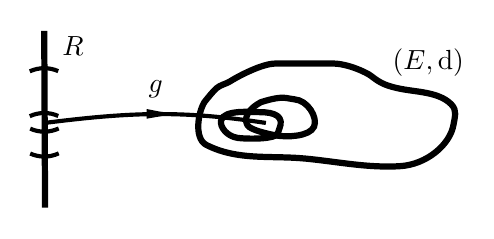
\begin{tikzpicture}[x=0.75pt,y=0.75pt,yscale=-0.6,xscale=0.8]
%uncomment if require: \path (0,300); %set diagram left start at 0, and has height of 300

%Straight Lines [id:da6857889427628007] 
\draw [line width=2.25]    (100,118) -- (100.5,260) ;
%Shape: Arc [id:dp022856158318092845] 
\draw  [draw opacity=0][line width=1.5]  (91.28,150.57) .. controls (94.04,148.9) and (96.97,148) .. (100,148) .. controls (102.93,148) and (105.76,148.84) .. (108.44,150.41) -- (100,208) -- cycle ; \draw  [line width=1.5]  (91.28,150.57) .. controls (94.04,148.9) and (96.97,148) .. (100,148) .. controls (102.93,148) and (105.76,148.84) .. (108.44,150.41) ;  
%Shape: Arc [id:dp8618858057031726] 
\draw  [draw opacity=0][line width=1.5]  (108.72,196.43) .. controls (105.96,198.1) and (103.03,199) .. (100,199) .. controls (97.07,199) and (94.24,198.16) .. (91.56,196.59) -- (100,139) -- cycle ; \draw  [line width=1.5]  (108.72,196.43) .. controls (105.96,198.1) and (103.03,199) .. (100,199) .. controls (97.07,199) and (94.24,198.16) .. (91.56,196.59) ;  
%Shape: Arc [id:dp19616233704048058] 
\draw  [draw opacity=0][line width=1.5]  (108.72,216.43) .. controls (105.96,218.1) and (103.03,219) .. (100,219) .. controls (97.07,219) and (94.24,218.16) .. (91.56,216.59) -- (100,159) -- cycle ; \draw  [line width=1.5]  (108.72,216.43) .. controls (105.96,218.1) and (103.03,219) .. (100,219) .. controls (97.07,219) and (94.24,218.16) .. (91.56,216.59) ;  
%Shape: Arc [id:dp41839281673222306] 
\draw  [draw opacity=0][line width=1.5]  (91.28,186.57) .. controls (94.04,184.9) and (96.97,184) .. (100,184) .. controls (102.93,184) and (105.76,184.84) .. (108.44,186.41) -- (100,244) -- cycle ; \draw  [line width=1.5]  (91.28,186.57) .. controls (94.04,184.9) and (96.97,184) .. (100,184) .. controls (102.93,184) and (105.76,184.84) .. (108.44,186.41) ;  
%Shape: Regular Polygon [id:dp27683657588229815] 
\draw  [line width=2.25]  (272.77,144.33) .. controls (261.5,144.33) and (250.23,144.12) .. (238.96,144.33) .. controls (231.27,144.47) and (217.48,153.96) .. (211.91,158.63) .. controls (209.41,160.73) and (205.86,161.55) .. (203.8,164.08) .. controls (201.21,167.24) and (199.2,170.83) .. (197.03,174.3) .. controls (193.2,180.42) and (189.44,204.16) .. (197.71,209.71) .. controls (216.61,222.41) and (235.93,217.93) .. (257.22,220.61) .. controls (276.7,223.07) and (294.22,228.2) .. (314.02,226.74) .. controls (330.44,225.53) and (344.51,209.23) .. (346.48,193.37) .. controls (347.22,187.45) and (348.9,182.09) .. (345.13,177.02) .. controls (337.39,166.62) and (323.57,167.37) .. (312.67,164.08) .. controls (304,161.46) and (301.35,158.81) .. (296.44,153.86) .. controls (294.23,151.64) and (282.2,143.76) .. (272.77,144.33) -- cycle ;
%Curve Lines [id:da367767170262597] 
\draw [line width=1.5]    (100.25,192) .. controls (153.5,183) and (183.5,182) .. (233.5,192) ;
\draw [shift={(177.27,184.98)}, rotate = 181] [fill={rgb, 255:red, 0; green, 0; blue, 0 }  ][line width=0.08]  [draw opacity=0] (15.6,-3.9) -- (0,0) -- (15.6,3.9) -- cycle    ;
%Shape: Polygon Curved [id:ds9549073342099108] 
\draw  [line width=2.25] [line join = round][line cap = round] (229.83,183.33) .. controls (224.98,183.33) and (208,181.03) .. (206.5,190) .. controls (205.65,195.09) and (209.94,202.74) .. (216.5,204) .. controls (220.72,204.81) and (235.1,205.3) .. (239.5,202) .. controls (240.94,200.92) and (240.93,198.7) .. (241.5,197) .. controls (244.89,186.82) and (239.01,183.33) .. (229.83,183.33) -- cycle ;
%Shape: Regular Polygon [id:dp6827950932437457] 
\draw  [line width=2.25]  (230.5,175.33) .. controls (219.5,183.33) and (221.21,191.42) .. (222.5,194) .. controls (224.38,197.76) and (234.91,200.85) .. (239.5,202) .. controls (245.82,203.58) and (259.8,203.09) .. (262.5,195) .. controls (264.86,187.91) and (258.89,173.7) .. (250.5,173) .. controls (246.13,172.64) and (244.5,169.33) .. (230.5,175.33) -- cycle ;

% Text Node
\draw (109,120.4) node [anchor=north west][inner sep=0.75pt]    {$\mathbb{R}$};
% Text Node
\draw (308,130) node [anchor=north west][inner sep=0.75pt]    {$( E,\mathrm{d})$};
% Text Node
\draw (161,155.4) node [anchor=north west][inner sep=0.75pt]    {$g$};


\end{tikzpicture}
\caption{Example on $\RR$}
    \end{figure}
\end{exampleenv}
\begin{exampleenv}
    Let $(G,\le)$ be a totally ordered set, $\mathcal{F}$ be the ordered topology on $G$. It is generated by $\{G_{>a}\mid a\in g\}\cup\{G_{<b}\mid b\in G\}$. If $l\in G$, then $\mathcal{V}_x(\mathscr{T})$ is generated by 
    $$S_l:=\{G_{>a}\mid a<l\}\cup\{G_{<b}\mid l<b\}.$$
    Assume that $(G,\le)$ is order complete. Let $f:X\longrightarrow G$ be a mapping and $\mathcal{F}$  be  a non-degenerate filter on $X$.
    \newline
    (1) Assume that $f$ converges to $l$ along $\mathcal{F}$. $\forall a< l, \ U_a:=f^{-1}\left(G_{>a}\right)\in \mathcal{F}$. $\forall x\in U_a, f(x)>a$. So $\liminf_{\mathcal{F}}f\ge a$. If $\sup\left(G_<l\right)=l$, then $\liminf_{\mathcal{F}}f\ge l.$ If $\sup\left(G_{<l}\right)<l$, we denote $a=\sup\left(G_{<l}\right)$. $\forall a\in U_a, f(x)\ge l$. So $\liminf_{\mathcal{F}}f\ge l$. Similarly, $\liminf_{\mathcal{F}}f\le l$. So $f$ admits $l$ as its limit.
    \newline
    (2) Assume that $\limsup_{\mathcal{F}}f=\liminf_{\mathcal{F}}f=l$. 
    $$\liminf_{\mathcal{F}}f=l\Rightarrow \sup_{U\in \mathcal{F}}f^i(U)=l, \forall a<l, \exists U\in \mathcal{F}, f^i(U)>a, f^{-1}(G_{>a})\in \mathcal{F}.$$
    $$\limsup_{\mathcal{F}}f=l\Rightarrow \forall b>l, f^{-1}(G_{<b})\in \mathcal{F}.$$
    Therefore, $f$ converges to $l$ along $\mathcal{F}$.
\end{exampleenv}


\section{Continuity}
\begin{definitionenv}
    Let $(X,\mathscr{T}_X)$ and $(Y,\mathscr{T}_Y)$ be topological spaces, $f$ be a function from $X$ to $Y$, and $p\in \mathrm{Dom}(f)$. If for any neighborhood $U$ of $f(p)$, there exists a neighborhood $V$ of $p$ such that 
    $$f(V)\subseteq U,$$
    then we say that the function $f$ is \textbf{continuous} at the point $p$. 
    
    If $f$ is continuous at any $p\in \mathrm{Dom}(f)$, then we say that $f$ is \textbf{continuous}.
\end{definitionenv}
\begin{remark}
    \ \newline
    (1) The continuity of $f$ at $p$ is equivalent to:
    $$\underset{x\rightarrow p}{\lim_{x\in \mathrm{Dom}(f)}}f(x)=f(p),$$
    namely, $f$ converges to $f(p)$ when $x$ tends to $p$.
    \newline
    (2) Let $\mathcal{V}_{f(p)}\left(\mathscr{T}_Y\right)$ and $\mathcal{V}_{p}\left(\mathscr{T}_X\right)$ be filters of neighborhoods of $f(p)$ and $p$ respectively. Let $\mathcal{B}_p$ be a filter basis that generates $\mathcal{V}_p\left(\mathscr{T}_X\right)$. Let $S_{f(p)}$ be a subset of $\mathcal{V}_{f(p)}\left(\mathscr{T}_Y\right)$ that generates $\mathcal{V}_{f(p)}\left(\mathscr{T}_Y\right)$. Then the continuity of $f$ at $p$ is equivalent to:
    $$\forall U\in S_{f(p)},\ \exists V\in \mathcal{B}_p,\ f(V)\subseteq U.$$
    In the case where $X$ and $Y$ are metric spaces, this condition becomes:
    $$\forall \varepsilon >0,\ \exists \delta>0,\ \forall x\in \mathrm{Dom}(f),\ \mathrm{d}(x,p)<\delta\Rightarrow \mathrm{d}(f(x),f(p))<\varepsilon.$$
\end{remark}
\begin{propositionenv}
    Let $(X,\mathscr{T}_X),\ (Y,\mathscr{T}_Y),\ (Z,\mathscr{T}_Z)$ be topological spaces. $f: X\longrightarrow Y$, $g: Y\longrightarrow Z$ be functions. $p\in \mathrm{Dom}(g\circ f)$. Assume that $f$ is continuous at $p$ and $g$ is continuous at $f(p)$. Then $g\circ f$ is continuous at $p$.
\end{propositionenv}
\begin{proofenv}
    Let $U$ be a neighborhood of $g\left(f\left(p\right)\right)$. Since $g$ is continuous at $f(p)$, there exists a neighborhood $V$ of $f(p)$ such that $g(V)\subseteq U$. Since $f$ is continuous at $p$, there exists a neighborhood $W$ of $p$, such that $f(W)\subseteq V$. Hence $g\left(f\left(W\right)\right)\subseteq g\left(V\right)\subseteq U.$ So $g\circ f$ is continuous at $p$.
\end{proofenv}
\begin{exampleenv}
    Let $\left(X,\mathscr{T}_X\right)$ be a topological space. Then $\mathrm{Id}_X$ and constant mapping are continuous.
\end{exampleenv}
\begin{theoremenv}
Let $\left(X,\mathscr{T}_X\right)$, $\left(Y,\mathscr{T}_Y\right)$ be topological spaces, $f:X\longrightarrow Y$ a function, $p\in \mathrm{Dom}(f)$. Consider the following conditions:
\newline
(1) $f$ is continuous at $p$.
\newline
(2) For any $(x_n)_{n\in \NN}\in \mathrm{Dom}(f)^{\NN}$, if $\dis \lim_{n\rightarrow \infty}x_n=p$, then 
$$\lim_{n\rightarrow \infty}f(x_n)=f(p).$$
One has (1)$\Rightarrow$(2). If $p$ has a countable basis of neighborhoods, (2)$\Rightarrow$(1).
\end{theoremenv}
\begin{proofenv}
    Let $(x_n)_{n\in\NN}\in \mathrm{Dom}(f)^{\NN}$ such that $\dis \lim_{x\rightarrow \infty}x_n=p$. $f$ is continuous at $p$, so for any neighborhood $U$ of $f(p)$, there exists a neighborhood $V$ of $p$, such that $f(V)\subseteq U$. Since $\dis \lim_{n\rightarrow \infty}x_n=p$, there exists $N\in \NN$, so that for any $n\in \NN_{>N},\ x_n \in V$. Hence for any $n\in \NN_{>N}$, $f(x_n)\in U$. Hence $\dis \lim_{n\rightarrow \infty}f(x_n)=f(p)$.

    Assume that $p$ has a countable basis of neighborhood. Let $(W_n)_{n\in \NN}$ be a sequence of neighborhood of $p$, such that $\{W_n\mid n\in \NN\}$ forms a neighborhood basis. For $n\in \NN$, 
    $$V_n:=\bigcap_{i\in \NN_{\le n}}W_i.$$
    $V_n$ is a neighborhood of $p$. If $f$ is not continuous at $p$, then there exists an neighborhood of $p$, $U$, such that 
    $$\forall n\in \NN,\ f(V_n)\nsubseteq U.$$
    We pick $x_n\in V_n$ but $f(x_n)\notin U.$ For any neighborhood $V$ of $p$, there exists $N\in \NN$ such that $V_N\subseteq V$, so that $x_n\in V$ for any $n\in \NN_{>N}$. Hence, $x_n$ converges to $p$. But $f(x_n)$ cannot converge to $f(p)$.
\end{proofenv}
\begin{lemmaenv}
    Let $(X,\mathscr{T}_X)$ be a topological space. $V\subseteq X$. If $\forall p\in V$, $V$ is a neighborhood of $p$, then $V\in \mathscr{T}_X$. In fact $\forall p\in V$, there exists $W_p\in \mathscr{T}_X$, $p\in W_p\subseteq V$. Hence 
    $$V=\bigcup_{p\in V}\{p\}\subseteq \bigcup_{p\in V} W_p\subseteq V.$$
\end{lemmaenv}
\begin{propositionenv}
    Let $\left(X,\mathscr{T}_X\right)$, $\left(Y,\mathscr{T}_Y\right)$ be topological spaces, $\mathcal{S}\subseteq\mathscr{T}_Y$, $\mathcal{S}$ generates $\mathscr{T}_Y$. The following statements are equivalent:
    \newline
    (1) $f$ is continuous.
    \newline
    (2) For any $U\in \mathscr{T}_Y$, $f^{-1}(U)\in \mathscr{T}_X$.
    \newline
    (3) For any $U\in \mathcal{S}$, $f^{-1}(U)\in \mathscr{T}_X$.
\end{propositionenv}
\begin{proofenv}
    \ \newline
    (1)$\Rightarrow$(2): For any $p\in f^{-1}(U)$, one has $f(p)\in U$. Hence, there is a neighborhood $V_p$ of $p$, $f(V_p)\subseteq U$, or equivalently $V_p\subseteq f^{-1}(U)$. Therefore, $f^{-1}(U)\in \mathscr{T}_X$.
    \newline
    (3)$\Rightarrow$(2): 
    $$\mathscr{T}_{Y}'=\left\{U\in \wp(Y)\mid f^{-1}(U)\in\mathscr{T}_X\right\}$$
    By definition, $\{\varnothing, Y\}\subseteq \mathscr{T}_{Y}'$. If $(U_1,U_2)\in \mathscr{T}_Y'\times\mathscr{T}_Y'$, then $f^{-1}(U_1\cap U_2)=f^{-1}(U_1)\cap f^{-1}(U_2)\in\mathscr{T}_X$. So $U_1\cap U_2\in \mathscr{T}_Y'$. $(U_i)_{i\in I}\in\left(\mathscr{T}_{Y}'\right)^I$, then 
    $$f^{-1}\left(\bigcup_{i\in I}U_i\right)=\bigcup_{i\in I}f^{-1}(U_i)\in \mathscr{T}_X.$$
    So $\mathscr{T}_Y'$ is a topology, by (3), $\mathcal{S}\subseteq \mathscr{T}_Y'\Rightarrow\mathscr{T}_Y\subseteq \mathscr{T}_Y'$.
\end{proofenv}



\section{Initial Topology}
\begin{definitionenv}
    Let $X$ be a set, $\left((Y_i,\mathscr{T}_i)\right)_{i\in I}$ a family of topological spaces, $\left(f_i:X\longrightarrow Y_i\right)_{i\in I}$ a family of mappings. We call \textbf{initial topology} on $X$ induced by $\left(f_i\right)_{i\in I}$ the topology generated by 
    $$\bigcup_{i\in I}\left\{f^{-1}_i(U_i)\mid U_i\in \mathscr{T}_i\right\}.$$
    It is the coarsest topology on $X$ making all $f_i$ continuous.
\end{definitionenv}
\begin{propositionenv}
    Let $\mathscr{T}$ be the initial topology on $X$ induced by $\left(f_i\right)_{i\in I}$. 
    \newline
    (1) $$\mathcal{B}= \left\{ \bigcap_{j\in J}f^{-1}_j(U_j)\mid J\subseteq I \text{ finite, }\left(U_j\right)_{j\in J}\in \prod_{j\in J}\mathscr{T}_j\right\}$$
    is topological basis that generates $\mathscr{T}$.
    \newline
    (2) Let $(Z,\mathscr{T}_Z)$ be topological space, $h:Z\longrightarrow X$ be a function and $p\in \mathrm{Dom}(f)$. Then $h$ is continuous at $p$ if and only if $\forall i\in I,\ f_i\circ h$ is continuous at $p$.
\end{propositionenv}
\begin{proofenv}
    \ \newline
    (1) Let 
    $$S=\bigcup_{i\in I}\left\{f^{-1}_{i}\left(U_i\right)\mid U_i\in \mathscr{T}_i\right\},$$
    $\mathcal{B}'$ be the set of the intersections of all finitely elements of $S$ (We have proved that $\mathcal{B}'$ is a basis of $\mathscr{T}$). $\mathcal{B}\subseteq\mathcal{B}'$. Let $i_1,\dots, i_n$ elements of $I$, $U_{i_k}\in \mathscr{T}_{i_k}$, $J=\{i_1,\dots,i_n\},\ j\in J$, $A_j=\left\{k\in\{1,\dots,n\}\mid i_k=j\right\}$, $\dis W_j=\bigcap_{k\in A_j}U_{i_k}$.
    $$\bigcap_{k=1}^{n}f^{-1}_{i_k}\left(U_{i_k}\right)=\bigcap_{j\in J}f^{-1}_{j}\left(W_j\right)\in \mathcal{B}.$$
    (2) Since $f_i$ is continuous at $p$, if $h$ is continuous then $\forall i\in I$, $f_i\circ h$ is continuous. Assume $\forall i\in I,\ f_i\circ h$ is continuous, then 
    $$\forall i\in I,\ \forall U_i\in \mathscr{T}_i,\ \left(f_i\circ h\right)^{-1}\left(U_i\right)=h^{-1}\left(f_i^{-1}\left(U_i\right)\right).$$
    Therefore, for any $V\in S$, $h^{-1}(V)\in \mathscr{T}_Z.$ Hence $h$ is continuous.
\end{proofenv}
\begin{exampleenv}
    Let $(X_i,\mathscr{T}_i)$ be topological spaces, $X=\prod_{i\in I}X_i$, $\pi_i:X\longrightarrow X_i$ be a projection. The initial topology on $X$ induced by $(\pi_i)_{i\in I}$ is called the \textbf{product topology}.
\end{exampleenv}



\section{Uniform Continuity}
\begin{definitionenv}
    Let $(X, \mathrm{d}_X),\ (Y,\mathrm{d}_Y)$ be semimetric spaces, $f:X\longrightarrow Y$ be a function, $\alpha \in \RR_{\ge0}$. If for any $(x_1,x_2)\in \mathrm{Dom}(f)^2$, $\mathrm{d}\left(f(x_1),f(x_2)\right)\le \alpha\cdot \mathrm{d}(x_1,x_2)$, then we say that $f$ is $\alpha$-Lipschitzian. If there exists $\alpha\in \RR_{\ge 0}$ such that $f$ is \textbf{$\alpha$-Lipschitzian}, then we say that $f$ is \textbf{Lipschitzian}. 

    If 
    $$\forall \varepsilon>0,\exists \delta>0,\ \forall (x_1,x_2)\in \mathrm{Dom}(f)^2,\ \mathrm{d}_X(x_1,x_2)<\delta\Rightarrow \mathrm{d}(f(x_1),f(x_2))<\varepsilon,$$
    then we say that $f$ is \textbf{uniformly continuous}.
\end{definitionenv}
\begin{propositionenv}
    Let $(X,\mathrm{d}_X),\ (Y,\mathrm{d}_Y)$ be semimetric spaces, $f:X\longrightarrow Y$ be a function. If $f$ is uniformly continuous, then $f$ continuous.
\end{propositionenv}
\begin{proofenv}
Let $p\in \mathrm{Dom}(f)$. For $\varepsilon>0$, there exists $\delta>0$ such that 
$$\forall (x_1,x_2)\in \mathrm{Dom}(f)^2,\ \mathrm{d}_X(x_1,x_2)<\delta\Rightarrow \mathrm{d}(f(x_1),f(x_2))<\varepsilon.$$
In particular, 
$$\forall x\in \mathrm{Dom}(f),\ \exists \delta>0,\ \mathrm{d}_X(x,p)<\delta\Rightarrow \mathrm{d}_Y(f(x),f(p))<\varepsilon.$$
\end{proofenv}
\begin{definitionenv}
    Let $K$ be a field, we call absolute value on $K$ any mapping,
    $$\left|\ \cdot\ \right|: K\longrightarrow \RR_{\ge 0},$$
    (1) $\forall a\in K,\ a=0_K$ if and only if $\left|a\right|=0.$
    \newline
    (2) $\forall (a,b)\in K\times K,\ \left|ab\right|=\left|a\right|\left|b\right|.$
    \newline
    (3) $\forall (a,b)\in K\times K,\ \left|a+b\right|\le \left|a\right|+\left|b\right|.$
    \newline
    The pair $(K,\left|\ \cdot\ \right|)$ is called a \textbf{valued field}.

\end{definitionenv}
\begin{exampleenv}
    Let $(K,\le)$ be a totally ordered field, then $\left|a\right|=\max\{-a,a\}$ is an absolute value on $K$.
\end{exampleenv}
\begin{exampleenv}
    Let $p$ be a prime number. Any non-zero rational number $\alpha$ can be written in the form
    $$\alpha=p^{\mathrm{ord}_p(\alpha)}\cdot\frac{m}{n},$$
    where, $\mathrm{ord}_p(\alpha)\in \ZZ,\ p\nmid mn$. If $\alpha=0$, we set (by convention) $\mathrm{ord}_p(\alpha)=+\infty.$

    \textbf{Properties:} 
    \newline
    (1) $\mathrm{ord}_p(\alpha\beta)=\mathrm{ord}_p(\alpha)+\mathrm{ord}_p(\beta)$.
    \newline
    (2) $\alpha=p^{\mathrm{ord}_p(\alpha)}\frac{m}{n},\ \beta=p^{\mathrm{ord}_p(\beta)}\frac{u}{v}$, $\mathrm{ord}_p(\alpha)>\mathrm{ord}_p(\beta)$, $p\nmid nvu$.
    $$\alpha+\beta=p^{\mathrm{ord}_p(\beta)}\frac{p^{\mathrm{ord}(\alpha)-\mathrm{ord}(\beta)}mv+nu}{nv}.$$
    (3) If $\mathrm{ord}(\alpha)=\mathrm{ord}(\beta)$, then $\mathrm{ord}_{p}(\alpha+\beta)\ge \mathrm{ord}_p(\alpha)=\mathrm{ord}_p(\beta).$
    $$\alpha+\beta=p^{\mathrm{ord}_p(\alpha)}\frac{mv+nu}{nv}.$$
\end{exampleenv}
\begin{propositionenv}
    The mapping 
    $$\left|\ \cdot\ \right|_{p}: \QQ\longrightarrow \RR_{\ge 0},$$
    $$\left\{\begin{matrix}
        &|\alpha|_p=p^{-\mathrm{ord}(\alpha)}, &\text{if } \alpha\neq0\\
        &|\alpha|_p=0, &\text{if } \alpha=0
    \end{matrix}\right.$$
    is an absolute value on $\QQ$.
\end{propositionenv}
\begin{proofenv}
    If $\alpha=0$, then $|\alpha|_p>0$. If $(\alpha,\beta)\in \QQ^2$, when $0\in \{\alpha,\beta\}$, then $\alpha\beta=0$ and $0=|\alpha\beta|_p=|\alpha|_p|\beta|_p$. When $0\notin\{\alpha,\beta\}$, 
    $$|\alpha\beta|_p=p^{-\mathrm{ord}_p(\alpha\beta)}=p^{-\mathrm{ord}_p(\alpha)-\mathrm{ord}_p(\beta)}= |\alpha|_p|\beta|_p.$$
    If $\alpha=0$, $|\alpha\beta|_p= |\beta|_p.$ If $\beta=0$, $|\alpha\beta|_p= |\alpha|_p.$, if $0\notin\{\alpha,\beta\}$,
    $$|\alpha+\beta|_p=p^{-\mathrm{ord}_p(\alpha+\beta)}\le p^{\max\{\mathrm{ord}_p(\alpha),\mathrm{ord}_p(\beta)\}}\le \max\{|\alpha|_p,|\beta|_p\}\le |\alpha|_p+|\beta|_p.$$
\end{proofenv}
\begin{remark}
    Let $(K,\left|\ \cdot\ \right|)$ be a valued field. If for any $(\alpha,\beta)\in K^2$ satisfies $|\alpha+\beta|\le \max\{|\alpha|,|\beta|\}$, we say that $(K,\left|\ \cdot\ \right|)$ is \textbf{non-archimedean}, otherwise, we say that $(K,\left|\ \cdot\ \right|)$ is \textbf{archimedean}. $(\RR,\left|\ \cdot\ \right|)$ and $(\QQ,\left|\ \cdot\ \right|)$ are archimedean.
\end{remark}
\begin{definitionenv}
    Let $(K,\left|\ \cdot \ \right|)$ be a valued filed, $V$ a vector spaced over $K$. We call \textbf{seminorm} on $V$ any mapping 
    $$|\!| \cdot |\!|:V\longrightarrow \RR_{\geq 0}$$ 
    that satisfies the following conditions:
    \newline
    (1) $\forall (a,x)\in K\times V,\ |\!|ax|\!|=|a|\cdot|\!|x|\!|$.
    \newline
    (2) $\forall (x,y)\in V\times V,\ |\!|x+y|\!|\le |\!|x|\!|+|\!|y|\!|.$
    \newline
    Note that (1) implies that $|\!|0_V|\!|=|0_K|\cdot|\!|0_V|\!|=0$.

    The pair $(V,|\!| \cdot |\!|)$ is called \textbf{seminormed vector space} \textit{over} $(K,\left|\ \cdot\ \right|)$. If $\forall(x,y)\in V\times V,\ |\!|x+y|\!|\le \max\{|\!|x|\!|,|\!|y|\!|\}$, then we say that $|\!|\cdot|\!|$ is \textbf{ultrametric}. If $\forall x\in V\cdot\{0\}$, $|\!|x|\!|>0$, then we say that $|\!| \cdot|\!|$ is a \textbf{norm} and $(V,|\!| \cdot |\!|)$ is a \textbf{normed vector space} \textit{over} $(K,\left|\ \cdot\ \right|)$.
\end{definitionenv}
\begin{exampleenv}
    $\mathrm{d}:V\times V\longrightarrow \RR_{\ge 0}$, $\mathrm{d}(x,y):=|\!|x-y|\!|$ is a semi-metric. 
\end{exampleenv}
\begin{exampleenv}
    Let $(K,\left|\ \cdot\ \right|)$ be a valued field.
    \newline
    (1) $(K,\left|\ \cdot\ \right|)$ is a normed vector space over $(K,\left|\ \cdot\ \right|)$. ($\mathrm{d}(x,y)=|x-y|$ is a metric.)
    \newline
    (2) Let $(V_1,|\!|\cdot|\!|_1),\dots, (V_n,|\!|\cdot|\!|_n)$ be seminormed vector spaces over $(K,\left|\ \cdot\ \right|)$, $V=V_1\oplus\dots\oplus V_n$.
    $$|\!|\cdot|\!|_{l^\infty}:V\longrightarrow \RR_{\ge0},\ (x_1,\dots,x_n)\longmapsto\max_{i\in\{1,\dots,n\}}|\!|x_i|\!|_{i},\ x_i\in V_i,\ i\in \{1,\dots,n\},$$
    $$|\!|\cdot|\!|_{l^1}:V\longrightarrow \RR_{\ge0},\ (x_1,\dots,x_n)\longmapsto\sum_{i\in\{1,\dots,n\}}|\!|x_i|\!|_{i},\ x_i\in V_i,\ i\in \{1,\dots,n\}.$$
    $\forall \lambda\in K, \ \forall (x_1,\dots,x_n)\in V,$ 
    \begin{align*}
        \pl \lambda(x_1,\dots,x_n)\pl_{l^\infty}&=\pl(\lambda\cdot x_1,\dots,\lambda x_n)\pl_{l^\infty}\\
        &=\max_{i\in\{1,\dots,n\}}\pl\lambda x_i\pl_i\\
        &=\max_{i\in\{1,\dots,n\}}\left|\lambda\right||\!| x_i|\!|_{i}\\
        &=|\lambda|\max_{i\in\{1,\dots,n\}}|\!|x_i|\!|_{i}\\
        &=|\lambda|\cdot |\!|(x_1,\dots,x_n)|\!|_{l^\infty}.
    \end{align*}
    \begin{align*}
        \pl \lambda(x_1,\dots,x_n)\pl_{l^1}&=\pl(\lambda\cdot x_1,\dots,\lambda x_n)\pl_{l^1}\\
        &=\sum_{i\in\{1,\dots,n\}}\pl\lambda x_i\pl_i\\
        &=\sum_{i\in\{1,\dots,n\}}\left|\lambda\right||\!| x_i|\!|_{i}\\
        &=|\lambda|\sum_{i\in\{1,\dots,n\}}|\!|x_i|\!|_{i}\\
        &=|\lambda|\cdot |\!|(x_1,\dots,x_n)|\!|_{l^1}.
    \end{align*}
    $\forall x=(x_1,\dots,x_n),\ y=(y_1,\dots,y_n)\in V$,
    \begin{align*}
        \pl x+y\pl_{l^\infty}&=\pl(x_1+y_1,\dots,x_n+y_n)\pl_{l^\infty}=\max_{i\in\{1,\dots,n\}}\pl x_i+y_i\pl_i\\
        &\le \max_{i\in\{1,\dots,n\}}\pl x_i\pl_i+\pl y_i\pl_i\le \pl x\pl_{l^\infty}+\pl y\pl_{l^\infty}.
    \end{align*}
    \begin{align*}
        \pl x+y\pl_{l^1}&=\sum_{i\in\{1,\ldots,n\}}\pl x_i+y_i\pl_i\\
        &\le \sum_{i\in\{1,\dots,n\}}\pl x_i\pl_i+\pl y_i\pl_i= \pl x\pl_{l^1}+\pl y\pl_{l^1}.
    \end{align*}
    (3) Let $(V,\pl\cdot\pl)$ be a seminormed vector space over $K$, $f:W\longrightarrow V$ be a $K$-linear mapping. We denote by $\pl\cdot\pl_f$ the mapping $W\longrightarrow \RR_{\ge 0}$ define as 
    $$\forall x\in W, \ \pl x\pl_f:=\pl f(x)\pl.$$
    $\forall (\lambda,x)\in K\times W$, 
    $$\pl \lambda x\pl_f=\pl f(\lambda x)\pl =\pl \lambda f(x)\pl =\left|\lambda\right|\cdot\pl f(x)\pl=\lambda \pl x\pl_f.$$
    $\forall (x,y)\in W\times W$, 
    $$\pl x+y\pl_f=\pl f(x+y)\pl=\pl f(x)\pl+\pl f(y)\pl\le \pl x\pl_f+\pl y\pl_f.$$
    Therefore, $\pl\cdot\pl_f$ is a seminorm on $W$, called the \textbf{seminorm} \textit{induced by (the $K$-linear) mapping $f$}.
    \newline
    (4) Let $(V,\left|\ \cdot\ \right|)$ be a seminormed vector space over $K$, let $\pi:V\longrightarrow E$ be a surjective $K$-linear mapping. We denote by $\pl\cdot\pl_\pi$ the mapping
    $$E\longrightarrow \RR_{\ge 0},$$
    $$\alpha\longmapsto \inf_{x\in \pi^{-1}(\alpha)}\pl x\pl.$$
    If $(\lambda,\alpha)\in K\times E$,
    $$\pl \lambda\alpha\pl_\pi=\inf_{x\in \pi^{-1}(\lambda\alpha)}\pl x \pl=\inf_{x\in \pi^{-1}(\alpha)}\left|\lambda\right|\pl x\pl=\left|\lambda\right|\pl\alpha\pl_\pi.$$
    If $(\alpha,\beta)\in E\times E,$
    \begin{align*}
         \pl\alpha+\beta\pl_\pi=\inf_{z\in\pi^{-1}(\alpha+\beta)}\pl z\pl &=\inf_{(x,y)\in \pi^{-1}(\alpha)\times\pi^{-1}(\beta)}\pl x+y\pl \\
         &\le\inf_{(x,y)\in \pi^{-1}(\alpha)\times\pi^{-1}(\beta)}\pl x\pl +\pl y\pl\\
         &=\inf_{x\in \pi^{-1}(\alpha)}\pl x\pl+\inf_{y\in \pi^{-1}(\beta)}\pl y\pl.
    \end{align*}
    Hence $\pl\cdot\pl_\pi$ is a seminorm on $E$ called the \textbf{quotient seminorm} \textit{of $\pl\cdot\pl$ induced by $\pi$.} 
\end{exampleenv}
\begin{propositionenv}
    Let $(V,\pl\cdot\pl)$ be a seminormed vector space over a valued field $(K,\left|\ \cdot\ \right|)$.
    \newline
    (1) For any $a\in V$, the mapping $\tau_a:V\longrightarrow V,\ \tau_a(x)=x+a$ is $1$-Lipschitzian.
    \newline
    (2) For any $\lambda\in K$, the mapping $m_\lambda:V\longrightarrow V,\ m_\lambda(x):=\lambda\cdot x$ is $\lambda$-Lipschitzian.
    \newline
    (3) The mapping $\pl\cdot\pl: V\longrightarrow \RR$ is $1$-Lipschitzian.
\end{propositionenv}
\begin{proofenv}
    \ \newline
    (1) $\forall(x,y)\in V\times V,\ \pl \tau_a(x)-\tau_a(y)\pl=\pl(x+a)-(y+a)\pl=\pl x-y\pl$.
    \newline
    (2) $\forall (x,y)\in V\times V,\ \pl m_\lambda(x)-m_\lambda(y)\pl=\pl\lambda x-\lambda y\pl=\left|\lambda\right|\pl x-y\pl $.
    \newline
    (3) $\forall (x,y)\in V\times V,\ \pl x\pl =\pl (x-y)+y\pl\le\pl y\pl+\pl x-y\pl$. So $\pl x\pl -\pl y\pl \le \pl x-y\pl.$ Similarly, $\pl y\pl -\pl x\pl \le \pl y-x\pl.$ Hence,
    $$\left|\pl x\pl-\pl y\pl\right|\le \pl x-y\pl.$$
\end{proofenv}
\begin{definitionenv}
    $(E,\pl\cdot\pl_E),(F,\pl\cdot\pl_F)$ be two seminormed vector spaces over a valued field $(K,\left|\ \cdot\ \right|)$, and $\varphi$ a $K$-linear mapping from $E$ to $F$. We define $\pl\varphi\pl\in \left[0,+\infty\right]$  as
    $$\pl\varphi\pl:=\sup_{x\in E,\ \pl x\pl_E\neq 0}\frac{\pl\varphi(x)\pl_F}{\pl x\pl_E}.$$
    In the case where $\pl x_E\pl=0$, for any $x\in E$, by convention, $\pl\varphi(x)\pl$ is defined to be $0$. If $\pl \varphi\pl<+\infty$, we say that $\varphi$ is bounded. We denote by $\mathscr{L}(E,F)$ the set of all bounded $K$-linear mappings from $E$ to $F$.
\end{definitionenv}
\begin{remark}
    In the case when $(E,\pl \cdot\pl_E)=(K,\pl\cdot\pl) $, 
    $$\pl\varphi\pl=\sup_{x\in\mathcal{B}(0,1)}\pl\varphi(x)\pl_{F}.$$
\end{remark}
\begin{propositionenv}
    \ \newline
    (1) For any $\varphi\in\mathscr{L}(E,F)$ be the mapping $\varphi$ is $\pl\varphi\pl$-Lipschitzian. In particular, $\varphi$ is continuous.
    \newline
    (2) Suppose that there exists $\lambda\in K$, such that $|\lambda|>1$. If $\varphi: E\longrightarrow F$  is continuous at $0_E$, then $\varphi\in \mathscr{L}(E,F)$.
\end{propositionenv}
\begin{proofenv}
    For any $(x,y)\in E\times E$:
    \newline
    (1) $\pl\varphi(x)-\varphi(y)\pl_{F}=\pl\varphi(x-y)\pl_{F}\le \pl\varphi\pl\pl x-y\pl_{E}$.
    \newline
    (2) $\mathcal{B}(0_F,1):=\{\alpha\in F\mid \pl\alpha\pl_{F}<1\}$ is a neighborhood of $0_F$. There exists $\varepsilon>0$ such that 
    $$\varphi(\overline{\mathcal{B}}(0_E,\varepsilon))\subseteq\mathcal{B}(0_F,1)$$
    where $$\overline{\mathcal{B}}(0_E,\varepsilon):=\{x \in E\mid \pl x\pl_E<\varepsilon\}.$$
    Let $x\in E\backslash \{0\}$, there exists $n\in \ZZ$, such that $\pl\lambda ^n x\pl_E=\left|\lambda\right|^n\pl x\pl_E<\varepsilon$ and $\pl \lambda^{n+1}x\pl_{E}=\left|\lambda\right|^{n+1}\pl x\pl_E\ge \varepsilon$. Thus,
    $$\pl \varphi(x)\pl_F=\pl \lambda^{-n}\varphi(\lambda^n x)\pl_{F}=\left|\lambda\right|^{-n}\pl \varphi(\lambda^n x)\pl_{F}\le \left|\lambda\right|^{-n}\le\frac{\left|\lambda\right|}{\varepsilon}\pl x\pl_E.$$
    Therefore, $\pl\varphi\pl\le \frac{\lambda}{\varepsilon}$.
\end{proofenv}
\begin{propositionenv}
    Let $(E,\pl\cdot\pl_E),(F,\pl\cdot\pl_F)$ be two seminormed vector spaces over a valued field $(K,\left|\ \cdot\ \right|)$. Then $\mathscr{L}(E,F)$ is a vector subspace of $F^E$, and $\pl\cdot\pl$ is a seminorm on $\mathscr{L}(E,F)$, called the operator seminorm.
\end{propositionenv}
\begin{proofenv}
    Let $\varphi,\psi$ be to $K$-linear mappings from $E$ to $F$. For any $x\in E$, such that $\pl x\pl_E\neq0$.
    \begin{align*}
        \pl(\varphi+\psi)(x)\pl_F=&\pl\varphi(x)+\pl\psi(x)\pl_F\le \pl\varphi(x)\pl_F+\pl\psi(x)\pl_F\\
        \le& \pl\varphi\pl\pl x\pl_E+\pl\psi\pl\pl x\pl_E=\left(\pl\varphi\pl+\pl\psi\pl\right)\pl x\pl_E.
    \end{align*}
    $$\pl\varphi+\psi\pl\le\pl\varphi\pl+\pl\psi\pl.$$
    So, $\varphi,\psi\in \mathscr{L}(E,F)\Rightarrow \varphi+\psi\in \mathscr{L}(E,F)$.
    Let $\lambda\in K^\times$ and $\varphi\in \mathscr{L}(E,F)$, for any $x\in E$, $\pl x\pl _E\neq0$. One has 
    $$\pl (\lambda\varphi)(x)\pl_{F}=\pl\lambda\cdot\varphi(x)\pl_F=\left|\lambda\right|\pl\varphi(x)\pl_F \le \left|\lambda\right|\pl\varphi\pl\pl x\pl_E.$$
    So, $\pl\lambda\pl\le\left|\lambda\right|\pl\varphi\pl$, $\lambda\varphi\in \mathscr{L}(E,F)$. So $\mathscr{L}(E,F)$ is a vector subspace of $F^E$. Note that we can apply to $\lambda^{-1}$ and $\lambda\varphi$ and get 
    $$\pl \lambda^{-1}\cdot\lambda\varphi\pl=\pl\varphi\pl\le \left|\lambda^{-1}\right|\pl\lambda\varphi\pl=\left|\lambda\right|^{-1}\pl\lambda\varphi\pl,\ \left|\lambda\right|\le\pl\lambda\varphi\pl.$$
    Hence, $\left|\lambda\right|\pl\varphi\pl=\pl\lambda\varphi\pl$ and therefore $\pl\cdot\pl$ is a seminorm on $\mathscr{L}(E,F)$.
\end{proofenv}
\begin{definitionenv}
    Let $E$ be a vector space over $K$, and $\pl\cdot\pl_1$ and $\pl\cdot\pl_2$  be seminorms on $E$. We say that $\pl\cdot\pl_1$ and $\pl\cdot\pl_2$ are equivalent, if there exists $c_1, c_2\in \RR_{>0}$ such that 
    $$\forall x\in E,\ c_1\pl x\pl_1\le\pl x\pl_2\le c_2\pl x\pl_1.$$
\end{definitionenv}
\begin{propositionenv}
    Let $E$ be a vector space over $K$, and $\pl\cdot\pl_1$ and $\pl\cdot\pl_2$  be seminorms on $E$. If $\pl\cdot\pl_1$ and $\pl\cdot\pl_2$ are equivalent, then they define the same topology on $E$.
\end{propositionenv}
\begin{proofenv}
    Let $\mathscr{T}_1$ and $\mathscr{T}_2$ to be the topologies defined by $\pl\cdot\pl_1$ and $\pl\cdot\pl_2$, respectively. Then 
    $$\mathrm{Id}_E:(E,\mathscr{T}_1)\longrightarrow(E,\mathscr{T}_2)$$
    is bounded. So it is continuous, so $\mathscr{T}_2\subseteq\mathscr{T}_1$. Similarly, $\mathscr{T}_1\subseteq\mathscr{T}_2$.
\end{proofenv}
\begin{propositionenv}
    Let $n\in\NN_{\ge 1}$, and $(X_i,\mathrm{d}_i),\ i\in\{1,2,\ldots,n\}$ be $n$ seminormed vector spaces over $K$. Let $\dis X=\prod_{i=1}^nX_i$ and
    $$\mathrm{d}:X\times X\longrightarrow \RR_{\ge 0},$$
    $$\mathrm{d\left((x_1,\ldots,x_n),(y_1,\ldots,y_n)\right)}\longmapsto \max_{i\in\{1,\ldots,n\}}\mathrm{d}_i(x_i,y_i).$$
    Then $\mathrm{d}$ is a semimetric on $X$, and the topology  induced by $\mathrm{d}$ is the product topology of $\mathscr{T}_{\mathrm{d}_i}$ (topology induced on $X_i$ by $\mathrm{d}_i$) $i\in\{1,\dots,n\}$.

\end{propositionenv}
\begin{proofenv}
    \ \newline
    (1) $\mathrm{d}\left((x_1,\dots,x_n),(x_1,\dots,x_n)\right)=\max_{i\in\{1,\dots,n\}}\mathrm{d}_i(x_i,x_i)=0$.
    \newline
    (2) \begin{align*}
        &\mathrm{d}\left((x_1,\dots,x_n),(y_1,\dots,y_n)\right)=\max_{i\in\{1,\dots,n\}}\mathrm{d}_i(x_i,y_i)\\
        =&\max_{i\in\{1,\dots,n\}}\mathrm{d}_i(y_i,x_i)=\mathrm{d}\left((y_1,\dots,y_n),(x_1,\dots,x_n)\right).
    \end{align*}
    (3) \begin{align*}
        &\mathrm{d}((x_1,\dots,x_n),(z_1,\dots,z_n))\\
        =&\max_{i\in\{1,\dots,n\}}\mathrm{d}_i(x_i,z_i)\\
        \le&\max_{i\in\{1,\dots,n\}}\mathrm{d}_i(x_i,y_i)+\max_{i\in\{1,\dots,n\}}\mathrm{d}_i(y_i,z_i)\\
        =&\mathrm{d}((x_1,\dots,x_n),(y_1,\dots,y_n))+\mathrm{d}((y_1,\dots,y_n),(z_1,\dots,z_n)).
    \end{align*}
    So $\mathrm{d}$ is a semimetric on $X$. For $i\in \{1,\dots,n\}$, $\mathscr{T}_i:=\mathscr{T}_{\mathrm{d}_i}$, where $\mathscr{T}_\mathrm{d}$ is the topology induced by $\mathrm{d}$. Let $\pi_i: X\longrightarrow X_i$ be the project mapping (continuous with the product topology on $X$.) For any $x=(x_1,\dots,x_n), y=(y_1,\dots,y_n)$ in $X$,
    $$\mathrm{d}(x,y)=\max_{i\in\{1,\dots,n\}}\mathrm{d}_i(x_i,y_i)=\max_{i\in\{1,\dots,n\}}\mathrm{d}_i(\pi_i(x),\pi_i(y)),$$
    have $\forall i\in\{1,\dots,n\}$, $\mathrm{d}_i(x_i,y_i)\le \mathrm{d}(x,y)$ 
    which implies that 
    $$\mathrm{Id}_X:(X,\mathscr{T}_\mathrm{d})\longrightarrow (X,\mathscr{T})$$
    is continuous. So $\mathscr{T}\subseteq\mathscr{T}_\mathrm{d}.$
    \begin{align*}
        \mathcal{B}((p_1,\dots,p_n),\varepsilon)=&\{(x_1,\dots,x_n)\mid \mathrm{d}((p_1,\dots,p_n),(x_1,\dots,x_n))<\varepsilon\}\\
        =&\prod_{i=1}^n\mathcal{B}(p_i,\varepsilon)\in\mathscr{T}.
    \end{align*}
\end{proofenv}



\section{Closed Subsets}
\begin{exampleenv}[Review of open subsets]
    In $\RR$, an interval of the form $\interval[open]{a}{b}$ is open, since $\interval[open]{a}{b}=\mathcal{B}(\frac{a+b}{2},\frac{b-a}{2})$. An interval of the form $\interval[open]{a}{+\infty}$ is open, since $\dis \interval[open]{a}{+\infty}=\bigcup_{n\in\NN_{\ge 1}}\interval[open]{a}{a+n}$.
\end{exampleenv}
\begin{definitionenv}
    Let $(X,\mathscr{T})$ be a topological space. We say a subset $Y$ of $X$ is \textbf{closed} if $X\setminus Y$ is open.
\end{definitionenv}
\begin{remark}
    \ \newline
    (1) $\varnothing$, $X$ are closed.
    \newline
    (2) If $F_1$, $F_2$ are closed subset of $X$, then $F_1\cup F_2$ is closed.
    \newline
    (3) If $(F_i)_{i\in I}$ is a non-empty family of closed subsets of $X$, then $\dis \bigcap_{i\in I}F_i$ is closed.
\end{remark}
\begin{exampleenv}
    Let $(a,b)\in \RR^2$, $a<b$, then $[a,b]\subseteq \RR^2$ is closed. Moreover, $\interval[open left]{-\infty}{a}$ is closed.
\end{exampleenv}
\begin{propositionenv}
    Let $(X,\mathscr{T}_X)$ and $(Y,\mathscr{T}_Y)$ be topological spaces, and $f:X\longrightarrow Y$ be a mapping, then the following statements are equivalent:
    \newline
    (1) $f$ is continuous.
    \newline
    (2) For any closed subset $F$ of $Y$, $f^{-1}(F)$ is a closed subset of $X$.
\end{propositionenv}
\begin{proofenv}
    \ \newline
    (1) $\Leftrightarrow$ (2): $f$ is continuous if and only if, for any open subset $U$ of $Y$, $f^{-1}(U)\in \mathscr{T}_X$. Let $F\subseteq Y$ be closed, then $Y\backslash F$ is open. So
    $f^{-1}(Y\backslash F)=X\backslash f^{-1}(F)$ is open, so $f^{-1}(F)$ is closed.
    \newline
    (2) $\Leftrightarrow$ (1): Let $U\in \mathscr{T}_Y$, then $F=Y\backslash U$ is closed, so $f^{-1}(F)=X\backslash f^{-1}(U)$ is closed. So $f^{-1}(U)\in \mathscr{T}_Y$.
\end{proofenv}
\begin{exampleenv}
    \ \newline
    In $\RR^2$, $\{(x,y)\in \RR^2\mid x\ge 1\}$ is closed. Since $\RR^2\backslash\{(x,y)\mid x\ge 1\}=\interval[open]{-\infty}{0}\times \RR$. Since $f(x,y)=x+y$ is continuous, then $f^{-1}(\interval[open right]{0}{+\infty})=\{(x,y)\in \RR^2\mid x+y\ge 0\}$ is closed.
\end{exampleenv}
\begin{exampleenv}
    Let $(X,\mathrm{d})$ be a semimetric space. Let $Y\subseteq X$, $Y\neq\varnothing$. We define, for any $x\in X$,
    $$\mathrm{d}(x,Y)=\inf_{y\in Y}\mathrm{d}(x,y)\in \RR_{\ge 0}.$$
\begin{figure}[H]
    
\begin{center}
        

\tikzset{every picture/.style={line width=0.75pt}} %set default line width to 0.75pt        

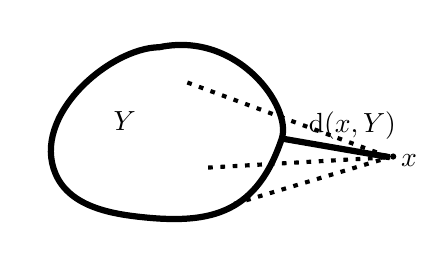
\begin{tikzpicture}[x=0.75pt,y=0.75pt,yscale=-1,xscale=1]
%uncomment if require: \path (0,300); %set diagram left start at 0, and has height of 300

%Shape: Polygon Curved [id:ds27882773645222514] 
\draw  [line width=2.25] [line join = round][line cap = round] (219.5,106) .. controls (195.45,106.4) and (157.57,139.15) .. (169.5,167) .. controls (176.48,183.3) and (197.45,186.5) .. (212.5,188) .. controls (244.94,191.24) and (266.64,185.58) .. (278.5,150) .. controls (283.51,134.98) and (257.5,98.09) .. (219.5,106) -- cycle ;
%Shape: Free Drawing [id:dp255407836209968] 
\draw  [line width=2.25] [line join = round][line cap = round] (332.17,158.67) .. controls (332.17,158.67) and (332.17,158.67) .. (332.17,158.67) ;
%Straight Lines [id:da009494640139930732] 
\draw [line width=2.25]    (278.5,150) -- (330.5,159) ;
%Straight Lines [id:da3200364645577044] 
\draw [line width=1.5]  [dash pattern={on 1.69pt off 2.76pt}]  (255.64,181.46) -- (330.5,159) ;
%Straight Lines [id:da7022259042728503] 
\draw [line width=1.5]  [dash pattern={on 1.69pt off 2.76pt}]  (233,123) -- (330.5,159) ;
%Straight Lines [id:da6184331447803212] 
\draw [line width=1.5]  [dash pattern={on 1.69pt off 2.76pt}]  (243,164) -- (330.5,159) ;

% Text Node
\draw (290,135.4) node [anchor=north west][inner sep=0.75pt]    {$\mathrm{d}( x,Y)$};
% Text Node
\draw (334.5,156.4) node [anchor=north west][inner sep=0.75pt]    {$x$};
% Text Node
\draw (196,135.4) node [anchor=north west][inner sep=0.75pt]    {$Y$};


\end{tikzpicture}
    \end{center}
    \caption{Definition of $\dd(\cdot, Y)$.}
\end{figure}
    The mapping $\dd(\cdot,Y): X\longrightarrow \RR$, $x\longmapsto \mathrm{d}(x,Y)$ is $1$-Lipschitzian.
    \newline
    Let $(x,x')\in X\times X$, $\forall y\in Y$,
    $$\dd (x,y)-\dd(x',y)\le \dd(x,x').$$
    Taking the infimum, we get 
    $$\dd(x,Y)-\dd(x',Y)\le \dd(x,x').$$
    By symmetry between $x$ and $x'$, $\dd(x',Y)-\dd(x,Y)\le \dd(x,x')$. So 
    $$|\dd(x,Y)-\dd(x',Y)|\le |\dd(x,x')|.$$
    For any $r>0$, define 
    $$B(Y,r):=\{x\in X\mid \dd(x,Y)< r\},$$
    $$\overline{B}(Y,r):=\{x\in X\mid \dd(x,Y)\le r\}$$
    $B(Y,r)$ is open, $\overline{B}(Y,r)$ is closed. If $Y=\{y\}$ is a one point set, $B(Y,r)$ and $\overline{B}(Y,r)$ are defined as $B(y,r)$ and $\overline{B}(y,r)$ respectively.
\end{exampleenv}
\begin{definitionenv}
    Let $(X,\mathscr{T})$ be a topological space. 
    \newline
    (1) Let $\mathcal{F}$ be a non-degenerate filter, an element $p\in X$ is called \textbf{adherent point} \textit{of} $\mathcal{F}$ if $\mathcal{F}\cup\mathcal{V}_p(\mathscr{T})$  generates a non-degenerate filter. ($\forall U\in \mathcal{F}$, $\forall V\in \mathcal{V}_p(\mathscr{T}), U\cap V\neq \varnothing.$) 
    \newline
    (2) Let $Y\subseteq X$. We say that $p\in X$ is an adherent point of $Y$ if it is an adherent point of the principal filter $\mathcal{F}_Y=\{U\subseteq X\mid Y\subseteq U\}$. (For any neighborhood $V$ of $p$, $Y\cap V\neq\varnothing$.) We denote by $\overline{Y} $ the set of all adherent points of $Y$ called the \textbf{closure} of $Y$. Clearly, $Y\subseteq \overline{Y}$.
\end{definitionenv}
\begin{propositionenv}
    Let $(X,\mathscr{T}_X)$ be a topological space, $Y\subseteq X$. Then $\overline{Y}$ is the smallest closed subset containing $Y$. Namely, 
    $$\overline{Y}=\bigcap_{\underset{Y\subseteq F}{F\subseteq X \text{ closed,}}} F.$$
\end{propositionenv}
\begin{proofenv}
    Let $p\in\overline{Y}$. If there exists a closed subset $F$ containing $Y$ such that $p\notin F$. So $p\in X\backslash F$. Hence $X\backslash F\in\mathcal{V}_p(\mathscr{T})$. So $\varnothing=(X\backslash Y)\cap Y\supseteq(X\backslash F)\cap Y\neq\varnothing$. Contradiction. Therefore,
    $$\overline{Y}\subseteq\bigcap_{\underset{Y\subseteq F}{F\subseteq X \text{ closed,}}} F.$$
    Suppose that $x\in X \backslash \overline{Y}$. There exists an open neighborhood $U$ of $x$ such that $U\cap Y=\varnothing$. So $x\notin F:=X\backslash U$. 
    \begin{figure}[H]
    

    \begin{center}
    
    




% Pattern Info
 
\tikzset{
pattern size/.store in=\mcSize, 
pattern size = 5pt,
pattern thickness/.store in=\mcThickness, 
pattern thickness = 0.3pt,
pattern radius/.store in=\mcRadius, 
pattern radius = 1pt}
\makeatletter
\pgfutil@ifundefined{pgf@pattern@name@_6i26so0vk}{
\pgfdeclarepatternformonly[\mcThickness,\mcSize]{_6i26so0vk}
{\pgfqpoint{0pt}{-\mcThickness}}
{\pgfpoint{\mcSize}{\mcSize}}
{\pgfpoint{\mcSize}{\mcSize}}
{
\pgfsetcolor{\tikz@pattern@color}
\pgfsetlinewidth{\mcThickness}
\pgfpathmoveto{\pgfqpoint{0pt}{\mcSize}}
\pgfpathlineto{\pgfpoint{\mcSize+\mcThickness}{-\mcThickness}}
\pgfusepath{stroke}
}}
\makeatother
\tikzset{every picture/.style={line width=0.75pt}} %set default line width to 0.75pt        
\usetikzlibrary{patterns}
\begin{tikzpicture}[x=0.75pt,y=0.75pt,yscale=-0.9,xscale=0.9]
%uncomment if require: \path (0,300); %set diagram left start at 0, and has height of 300

%Curve Lines [id:da7933044259634054] 
\draw [line width=3] [line join = round][line cap = round]   (348.5,134.67) .. controls (339.5,120.67) and (326.51,126.69) .. (317.77,122.24) .. controls (305.85,116.19) and (296.86,105.08) .. (284.58,99.9) .. controls (277.29,96.82) and (266.52,96.59) .. (259.41,97.42) .. controls (238.51,99.87) and (232.7,128.44) .. (223.37,143.96) .. controls (219.77,149.95) and (214.02,154.55) .. (208.49,158.24) .. controls (205.12,160.49) and (200.64,161.26) .. (197.05,163.2) .. controls (189.45,167.33) and (189.4,177.81) .. (194.19,184.3) .. controls (195.99,186.74) and (197.91,188.65) .. (200.48,190.51) .. controls (203.07,192.38) and (209.65,193.46) .. (212.5,193.61) .. controls (219.34,193.98) and (230.52,194.47) .. (238.24,192.37) .. controls (254.53,187.95) and (269.17,177.7) .. (286.3,176.24) .. controls (311.98,174.04) and (328.58,198.77) .. (354.95,195.47) .. controls (361.08,194.71) and (364.01,190.71) .. (366.4,185.54) .. controls (372.89,171.46) and (374.25,163.35) .. (364.68,148.93) .. controls (362.23,145.23) and (359.2,146.61) .. (348.5,134.67) -- cycle ;
%Curve Lines [id:da8598169086327346] 
\draw [line width=3] [line join = round][line cap = round] [dash pattern={on 3.38pt off 3.27pt}]  (353.47,124.59) .. controls (341.46,116.52) and (333.06,117.8) .. (322.64,112.22) .. controls (308.45,104.6) and (300.59,100.68) .. (285.96,94.18) .. controls (277.27,90.31) and (265.83,90.65) .. (257.36,91.7) .. controls (232.46,94.77) and (227.61,123.97) .. (216.17,143.2) .. controls (203.58,153.75) and (180.1,157.24) .. (181.82,172.76) .. controls (177.24,188.9) and (196.08,204.65) .. (199.47,204.85) .. controls (207.63,205.31) and (220.94,205.92) .. (230.15,203.29) .. controls (249.56,197.74) and (267,184.86) .. (287.41,183.01) .. controls (318.01,180.25) and (326.69,207.38) .. (358.11,203.24) .. controls (365.41,202.27) and (371.29,190.49) .. (374.13,184) .. controls (381.86,166.31) and (375.36,155.39) .. (363.96,137.27) .. controls (362.25,133.37) and (359.7,132.74) .. (353.47,124.59) -- cycle ;
%Shape: Rectangle [id:dp051984022647582284] 
\draw  [pattern=_6i26so0vk,pattern size=6pt,pattern thickness=0.75pt,pattern radius=0pt, pattern color={rgb, 255:red, 0; green, 0; blue, 0}][line width=3]  (172.41,81) -- (499.41,81) -- (499.41,238) -- (172.41,238) -- cycle ;
%Curve Lines [id:da10022472571045526] 
\draw [fill={rgb, 255:red, 255; green, 255; blue, 255 }  ,fill opacity=1 ][line width=3] [line join = round][line cap = round]   (457.5,136.33) .. controls (449.83,131.67) and (442.62,131.42) .. (433.5,132.33) .. controls (421.78,133.51) and (411.77,146.91) .. (415.5,159.33) .. controls (418.13,168.09) and (411.41,168.99) .. (429.41,181.99) .. controls (444.67,189.62) and (456.59,192.15) .. (467.5,170.33) .. controls (468.38,168.58) and (470.12,167.23) .. (470.5,165.33) .. controls (472.08,157.45) and (471.27,148.1) .. (466.5,143.33) .. controls (465.65,142.49) and (464.83,138.67) .. (457.5,136.33) -- cycle ;
%Shape: Free Drawing [id:dp9046103363043781] 
\draw  [line width=2.25] [line join = round][line cap = round] (442.83,163) .. controls (442.83,164.93) and (441.83,164.54) .. (441.83,163) ;

% Text Node
\draw (426,135.4) node [anchor=north west][inner sep=0.75pt]    {$U$};
% Text Node
\draw (448,153.4) node [anchor=north west][inner sep=0.75pt]    {$x$};
% Text Node
\draw (465,214.4) node [anchor=north west][inner sep=0.75pt]    {$\mathnormal{F}$};
% Text Node
\draw (509,189.4) node [anchor=north west][inner sep=0.75pt]    {$X$};
% Text Node
\draw (246.34,147.23) node [anchor=north west][inner sep=0.75pt]    {$Y$};
% Text Node
\draw (332.29,94.44) node [anchor=north west][inner sep=0.75pt]    {$\overline{Y}$};


\end{tikzpicture}
\end{center}
\caption{Closure}
\end{figure}
    Note that $F$ is closed and $F\supseteq Y$. Therefore, 
    $$X\backslash \overline{Y}\subseteq \bigcup_{\underset{Y\subseteq F}{F\subseteq X \text{ closed,}}} (X\backslash F).$$
    which leads to 
    $$\overline{Y}\supseteq X\backslash \left(\bigcup_{\underset{Y\subseteq F}{F\subseteq X \text{ closed,}}} (X\backslash F)\right)=\bigcap_{\underset{Y\subseteq F}{F\subseteq X \text{ closed,}}} F.$$


    


\end{proofenv}
\begin{definitionenv}
    Let $(X,\mathscr{T})$ be a topological space and $Y\subseteq X$. We denote by $Y^\circ$ the set of $p\in Y$ such that $Y$ is a neighborhood of $p$.
\end{definitionenv}
\begin{propositionenv}
    $Y^\circ$ is the least\footnote{largest} open subset of $X$ such that is contained in $Y$. Moreover,
    $$X\backslash Y^\circ=\overline{X\backslash Y}.$$
\end{propositionenv}
\begin{proofenv}
    $\forall y\in Y^\circ$, there exists $U_y\in\mathscr{T}$ such that $y\in U_y\subseteq Y$. Therefore, $\forall x\in U_y$, $Y$ is a neighborhood of $x$, hence, $U_y\subseteq Y^\circ$. We thus obtain 
    $$Y^\circ=\bigcup_{y\in Y^\circ}\{y\}\subseteq\bigcup_{y\in Y^\circ}U_y\subseteq Y^\circ.$$ 
    Hence $Y^\circ$ is open. 
    \newline
    If $U\subseteq Y$ is open, then $\forall x\in U$, $Y$ is a neighborhood of $x$. So $U\subseteq Y^\circ$. Therefore, $Y^\circ$ is the largest open subset that is contained in $Y$.
    $$X\backslash Y^\circ=X\backslash\bigcup_{\underset{U\subseteq Y}{U\in \mathscr{T}}}U=\bigcap_{\underset{U\subseteq Y}{U\in \mathscr{T}}}X\backslash U\overset{F=X\backslash U}{=}\bigcap_{\overset{ F\text{ closed}}{X\backslash Y\subseteq F}}F=\overline{X\backslash Y}.$$
\end{proofenv}
\begin{definitionenv}
    Let $(X,\mathscr{T})$ be a topological space. We equip $X\times X$ with the product topology, (a topological basis is given by $\{U\times V\mid (U,V)\in\mathscr{T}^2\}$) Let 
    $$\Delta_X\coloneq\{(x,x)\mid x\in X\}\subseteq X\times X.$$
    If $\Delta_X$ is closed, we say that $(X,\mathscr{T})$ is a \textbf{Hausdorff space}. (Or $(X,\mathscr{T})$ is separated.)
\end{definitionenv}
\begin{propositionenv}
    $(X,\mathscr{T})$ is a Hausdorff space if and only if $\forall (x,y)\in X\times X$, $x\neq y$, there exists $(U,V)\in \mathcal{V}_x(\mathscr{T})\times \mathcal{V}_y(\mathscr{T})$, such that $U\cap V=\varnothing$.
    
    \begin{figure}[H]
        
\centering
\tikzset{every picture/.style={line width=0.75pt}} %set default line width to 0.75pt        

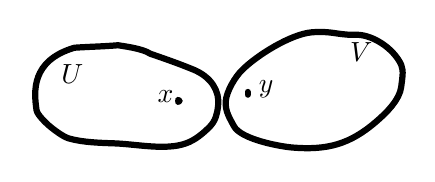
\begin{tikzpicture}[x=0.75pt,y=0.75pt,yscale=-0.8,xscale=0.8]


\draw  [line width=2.25]  (224.44,126.96) .. controls (219.83,123.68) and (206.96,122.25) .. (205.12,121.85) .. controls (194.97,122.69) and (188.44,122.69) .. (178.82,123.35) .. controls (152.52,131.1) and (154.39,149.97) .. (155.98,160.92) .. controls (156.39,163.75) and (161.97,169.05) .. (164.28,170.93) .. controls (165.91,172.26) and (171.78,176.91) .. (175.36,177.95) .. controls (183.78,180.38) and (194.17,180.63) .. (203.04,180.95) .. controls (216.42,181.44) and (233.91,185.31) .. (245.95,180.95) .. controls (251.7,178.87) and (255.95,175.14) .. (259.79,171.44) .. controls (263.87,167.5) and (264.7,163.37) .. (265.32,158.41) .. controls (266.44,149.5) and (261.25,140.86) .. (250.1,136.37) .. controls (244.45,134.1) and (239.14,131.99) .. (224.44,126.96) -- cycle ;

\draw  [line width=2.25] [line join = round][line cap = round] (241.29,154.82) .. controls (242.47,154.82) and (242.47,155.94) .. (241.29,155.94) ;

\draw  [line width=2.25] [line join = round][line cap = round] (283.12,149.98) .. controls (283.12,151.38) and (283.12,152.57) .. (283.12,151.18) ;

\draw  [line width=2.25]  (346.91,115.59) .. controls (337.26,115.59) and (333.41,113.15) .. (321.97,114.04) .. controls (309.18,115.03) and (288.4,128.06) .. (279.72,136.87) .. controls (275.62,140.79) and (270.45,149.55) .. (269.93,155.48) .. controls (269.4,161.54) and (272.49,166.06) .. (274.81,170.5) .. controls (279.05,178.61) and (302.95,182.87) .. (310.04,183.45) .. controls (331.33,185.19) and (344.79,181.39) .. (360.46,167.91) .. controls (366.25,162.94) and (374.78,154.86) .. (375.64,146.67) .. controls (376.06,142.68) and (377.29,137.4) .. (375.64,133.72) .. controls (371.01,123.41) and (357.25,114.6) .. (346.91,115.59) -- cycle ;

% Text Node
\draw (227,147.4) node [anchor=north west][inner sep=0.75pt]    {$x$};
% Text Node
\draw (288,141.4) node [anchor=north west][inner sep=0.75pt]    {$y$};
% Text Node
\draw (169,131.4) node [anchor=north west][inner sep=0.75pt]    {$U$};
% Text Node
\draw (343,118.4) node [anchor=north west][inner sep=0.75pt]    {$V$};


\end{tikzpicture}
\caption{Hausdorff space}
    \end{figure}
\end{propositionenv}
\begin{proofenv}
    \ \newline
    ``$\Rightarrow$'': If $(x,y)\in X\times X$, $x\neq y$, then $(x,y)\in (X\times X)\backslash \Delta_X$. There exists $ (U,V)\subseteq (X\times X)\backslash \Delta_X$, such that $(x,y)\in U\times V$, so $(U\times V)\cap \Delta_X=\varnothing$. Thus $U\cap V=\varnothing$. (If $p\in U\cap V$, then $(p,p)\in (U\times V)\cap \Delta_X$.)
    \newline
    ``$\Leftarrow$'': For any $(x,y)\in X\times X$, $x\neq y$, $\exists U\in \mathscr{T}$, $\forall V\in \mathscr{T}$, $x\in U, y\in V, U\cap V=\varnothing$. Then $(x,y)\in U\times V$ and $(U\times V)\cap \Delta_X=\varnothing$. So $\Delta_X$ is closed. 
\end{proofenv}
\begin{propositionenv}
    Let $(X,\mathscr{T})$ be a Hausdorff space. Let $\mathcal{F}$ be a non-degenerate filter on $X$. If $\mathcal{F}$ has a limit point\footnote{Let $(X,\mathscr{T})$ be a topological space and $\mathcal{F}$ be a filter on $X$. If $p\in X$ is such that $\mathcal{V}_p(\mathscr{T})\subseteq \mathcal{F}$, then we say that $p$ is a limit point of $\mathcal{F}$.}, then its limit point is unique.
\end{propositionenv}
\begin{proofenv}[By contradiction]
    Suppose that $x$ and $y$ are limit points of $\mathcal{F}$, $x\neq y$. Since $X$ is Hausdorff, $\exists (U,V)\in \mathscr{T}^2$, $x\in U,y\in V, U\cap V=\varnothing$. Since $x$ and $y$ are limit points of $\mathcal{F}$, $U\in\mathcal{F}, V\in \mathcal{F}$. This contradicts the hypothesis that $\mathcal{F}$ is non-degenerate.
\end{proofenv}
\begin{exampleenv}
    Any {\color{brown} metric space} is Hausdorff. 
    \newline
    Let $(X,\dd)$ be a metric space, $\forall (x,y)\in X\times X$, $x\neq y$, $\dd(x,y)>0$. Let $\varepsilon=\frac{\dd(x,y)}{2}$. $B(x,\varepsilon)\cap B(y,\varepsilon)=\varnothing.$ In fact, if $z\in B(x,\varepsilon)\cap B(y,\varepsilon)$,
    $$\dd(x,y)\le \dd(x,z)+\dd(z,y)<2\varepsilon=\dd(x,y).$$
\end{exampleenv}
\begin{propositionenv}
    Let $(X,\mathscr{T})$ be a topological space, $Y$ be a subset of $X$ and $p\in X$.
    \newline
    (1) Let $Z$ be a set and $f:Z\longrightarrow X$ be a mapping. Let $\mathcal{F}$ be a non-degenerate filter on $Z$. If $p$ is a limit of $f$ along $\mathcal{F}$, and if $f(Z)\subseteq Y$, then $p\in \overline{Y}$.
    \newline
    (2) Suppose that $p$ has a countable neighborhood basis. If $p\in \overline{Y}$, then there exists a sequence $(y_n)_{n\in\NN}$ in $Y$ that converges to $p$.
\end{propositionenv}
\begin{proofenv}
    \ \newline
    (1) $p$ is a limit of $f$ along $\mathcal{F}$ if and only if $\mathcal{V}_p(\mathscr{T})\subseteq f_*(\mathcal{F})$, or equivalently 
    $$\forall U\in \mathcal{V}_p(\mathscr{T}), f^{-1}(U)\in \mathcal{F}.$$
    $f(f^{-1}(U))\subseteq U\cap Y$, since $f(X)\subseteq Y$. Hence $U\cap Y\neq \varnothing$. So $p\in \overline{Y}.$
    \newline
    (2) Since $p$ has a countable neighborhood basis, there exists a decreasing sequence $V_0\supseteq V_1\supseteq\ldots$ of neighborhood of $p$ such that $\{V_n\mid n\in \NN\}$ forms a filter basis of $\mathcal{V}_p(\mathscr{T})$. For any $n\in \NN$, $V_n\cap Y=\varnothing$, we take $y_n\in V_n\cap Y$. The sequence $(y_n)_{n\in \NN}$ converges to $p$ since $\forall n\in \NN$, $\{y_k\mid k\in\NN,k\ge n\}\subseteq V_n$.
\end{proofenv}
\begin{exampleenv}
    Let $(X,\dd)$ be a semimetric space. $Y\subseteq X$, $\varepsilon>0$. If $(y_n)_{n\in\NN}$ is a sequence in $B(Y,\varepsilon)$, that converges to some $p\in X$, then 
    $$\lim_{n\rightarrow \infty}\dd(y_n,Y)=\dd(p,Y).$$
    Therefore, $\overline{B(Y,\varepsilon)}\subseteq \overline{B}(Y,\varepsilon):=\{x\in X\mid \dd(x,Y)\le \varepsilon\}$.
\end{exampleenv}
\begin{propositionenv}
    Let $(X,\dd)$ be a semimetric space, $Y\subseteq X$ be a closed subset. $\forall x\in X\backslash Y$, $\dd(x,Y)>0$.
\end{propositionenv}
\begin{proofenv}
    $X\backslash Y$ is open, so $\exists \varepsilon>0$ such that $B(X,\varepsilon)\subseteq{ X\backslash Y}$. So $\forall y\in Y$, $\dd(x,y)\ge \varepsilon$. Hence, $\dd(x,y)\ge \varepsilon$.
\end{proofenv}
\begin{corollaryenv}
    Let $(V,\pl\cdot\pl)$ be a semimetric space, $W$ be a closed vector subspace of $V$. $Q=V/W$. Then the quotient seminorm 
    $$\pl\cdot\pl_Q:Q\longrightarrow R,$$
    $$\alpha\longmapsto \inf_{x\in V,[x]=\alpha}\pl x\pl$$
    is a norm.
\end{corollaryenv}
\begin{proofenv}
    Let $\alpha\in Q\backslash{\alpha}$ and $x\in V$ such that $\alpha=[x]$. Since $\alpha\neq0, x\notin W$.
    $$0<\dd(x,W)\coloneq\inf_{y\in W}\pl x-y\pl=\inf_{\underset{[x']=\alpha}{x'\in V}}\pl x'\pl=\pl \alpha\pl_Q.$$
\end{proofenv}
\begin{propositionenv}
    If $(X,\mathscr{T})$ is a Hausdorff space, then, $\forall x\in X$, $\{x\}$ is closed.
\end{propositionenv}
\begin{proofenv}
    $\forall y\in X\backslash\{x\}$, $y\neq x$. So $\exists (U,V)\in \mathscr{T}\times\mathscr{T}$, $x\in U$, $y\in V$. $U\cap V=\varnothing$. So $V\subseteq X\backslash\{x\}$. Hence $X\backslash\{x\}$ is a neighborhood of $y$. 
\end{proofenv}
\begin{remark}
    Let $(V,\pl \cdot\pl)$ be a seminorm space. $W\subseteq V$, $Q=V/W$ and $\pl\cdot\pl_Q$ is the quotient seminorm. The mapping $\pi:V\longrightarrow Q, x\longmapsto [x]$  is continuous since $\pl[x]\pl_Q\le \pl x\pl$. If $\pl\cdot\pl_Q$ is a norm then $\{0_Q\}$ is closed (since $Q$ is Hausdorff). So $W=\pi^{-1}(\{0_Q\})=\ker(\pi)$ is closed. This shows that $\pl\cdot\pl_Q$ is a norm $\Leftrightarrow$ $W$ is closed.
\end{remark}



\section{Completeness}
\begin{definitionenv}
    Let $(X,\dd)$ be a semimetric space, $Y\subseteq X$, we define the diameter of $Y$ as $ \mathrm{diam}(Y)\coloneq\sup_{(x,y)\in Y^2}\dd(x,y)$. If $\mathrm{diam}(Y)<+\infty$, we say that $Y$ is \textbf{bounded}.
\end{definitionenv}
